
% Take extra care in avoiding ``expansion'' -- stick to ``evaluation''

\begin{abstract}
Despite the recent improvements in admissible heuristic search techniques
in classical planning, it is known that the the exponential growth of
search plateau in A* is unavoidable even under the optimistic assumption.
 % 
We investigate various existing myth on tiebreaking
strategies and propose simple yet effective methods for improving the
search performance within plateau.
 % 
 % 
 They do not depend on any particular heuristic, nor
 on multi-heuristic portfolio.
 They work even if the heuristic
 function no longer provides useful information.
 % Moreover, they do not even try to obtain any further information from
 % the domain.
 We empirically evaluate our strategies against state-of-the-art admissible planner.
\end{abstract}

\section{Introduction}
%Motivation: The Importance of the Last Frontier in A* and Domains with Large Plateaus
\label{sec-1}



%\subsubparagraph{\astar and perfect heuristics}

\astar is a standard search algorithm for finding an optimal-cost path 
from an initial state to some goal state in a search space represented as a graph \cite{hart1968formal}.
In each iteration, \astar selects and {\emph expands} a node $n$ from the OPEN priority queue.
\astar selects and expands the node which has the lowest $f$-cost, where $f(n)$ is the sum of  $g(n)$, the cost of the current path from the start state to $n$, and $h(n)$, a heuristic estimate of the cost from $n$ to a goal state.


%and has been used extensively in
%STRIPS planning in the recent years.
%\astar stores the search nodes into two priority queues called an
%\emph{open list}
%XXX The closed list is NOT a priority queue.
% and a \emph{closed list}. 

% On each iteration, \astar expands the open nodes with the
% smallest $f$ value and mark them as closed. Its successor nodes are
% accordingly inserted back to the open list or closed list, while
% sometimes the parent node is updated so that it has the shortest path
% from the initial state.

% Due to the space limitation,
% we assume the readers are already familiar with \astar
% and skip the details of the algorithm.

\astar returns an optimal solution when $h$ is admissible, i.e., when it
never overestimate the true distance to the goal $h^*$.




In order to guarantee the optimality of the solution, \astar expands all nodes with $f(n) < f^*$.
All nodes with $f(n) = k$ are be expanded before any node with $f(n)=m > k$ are expanded.
Thus, after all nodes with $f(n) < f^*$ have been expanded, \astar expands {\emph some} of the nodes with $f(n) = f^*$ until a goal node is found.
\astar never expands a node with $f(n) > f^*$.
Thus, the \emph{effective search space of \astar} is the set of nodes with 
$f(n) \leq f^*$.

Much of the work in the search literature as well as the domain-independent planning literature has focused on developing accurate, admissible heuristic functions, and 
by improving the quality of $h$, the size of the effective search space of \astar is reduced.


In many problems, the size of the set of nodes with $f(n)=f^*$
is quite large compared to the set of all nodes that can be considered by \astar, i.e., the set of nodes with $f(n) \leq f^*$.
\refig{fig:plateau-noh} plots the number of states with $f(n) = f^*$ (y-axis)
versus the number of states with $f(n) \leq f^*$
for a set of 1104 standard IPC problem instances from IPC98-IPC11.
Note that there are many instances where a large fraction of the nodes with $f(n) \leq f^*$ have $f(n)=f^*$.
For example, in the openstacks domain, all instances are on the y=x line, indicating that almost all states with $f(n) \leq f^*$ have cost $f^*$.
In such domains, the behavior of A* on the last frontier where $f(n)=f^*$ is critical -- the policy for determining which nodes to expand in the last frontier can have a significant impact on the performance of A*.

\begin{figure}[htb]
 \centering \relsize{-3}
 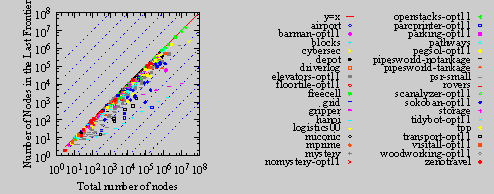
\includegraphics{tables/aaai16-frontier/aaai16-lmcut_frontier_noh-front-vs-expanded.pdf}
 \caption{
 Comparison of the number of the nodes $f=f^*$ compared to the
 total evaluation below $f\leq f^*$. Data were obtained by the result of
 Fast Downward with \lmcut on the standard benchmark instances. Both axes are
 logarithmic. Dotted lines represent $\times 10^n$ boundaries.}  \label{fig:plateau-noh}
\end{figure}

To date, there has not been much previous \emph{in-depth} work on the policy for searching the last frontier.
It is widely believed that among nodes with cost $f(n) = f^*$, ties should be broken according to $h(n)$, i.e., nodes with smaller $h$ values should be expanded first.
While this is a useful rule of thumb in many domains,
it turns out that the policy for breaking ties among nodes with the same $f$-cost requires more careful consideration.




% NOTE: Let's not overemphasize the Helmert and Rogers results on almost perfect heuristics.
% Although we'll certainly cite helmert2008good, we should not make helmrt2008good central
% to the motivation of the paper
% 
% Since the advent of delete-relaxation and abstraction heuristics in
% admissible Classical Planning, much of the interest was focused on improving
% the accuracy of these heuristic functions to prune more nodes from the
% search space.
% % 
% However, recent work by Helmert and Roger
% \shortcite{helmert2008good} claims that, even with an optimistic
% assumption of \emph{almost-perfect heuristics}, \astar still has an
% exponentially large plateau. They conclude that the further performance
% improvement requires the techniques orthogonal to the heuristic
% function, such as symmetry breaking, domain reduction, factored planning
% etc.

In this paper, we focus on the tiebreaking criteria of \astar.
%Sophisticated tiebreaking is a heuristic-agnostic improvement and thus 
%falls into above category of techniques.

[need better place for this] It trivially maintains admissibility because it works only within the
same f-value and does not alter the expansion order wrto f-value.

% such technique.
% tiebreaking strategy for \astar.
% Our tiebreaking strategies fall into this category.

% The attention to the search algorithm itself is relatively small since
% most literature depends on bare \astar.  This was because variations of
% best first search focus on different requirements, such as IDA* on
% linear space, WA*/Lazy-A*/GBFS/EHC on trading speed for optimality, RWA*
% on replanning, etc., and not on improving upon \astar itself.

% maintaining all of its charactristics: memory-greedy yet efficient
% optimal algorithm.

Specifically, we show several important findings regarding the
existing tiebreaking strategy for \astar as follows.
% 
First, in implementing the open list of \astar, priority queue based on
LIFO-buckets is more efficient than that of FIFO-buckets.
% 
Second, with LIFO-based implementation, $h$-based tiebreaking which
frequently appears in the heuristic search literatures have little
impact on the performance.
% 
Third, the LIFO-based bucket implementation and $h$-based tiebreaking
both share the greedy search pattern within the plateau of the
search space.
% 
Fourth, based on these observations, we propose a tiebreaking
method based on the \emph{depth} within the plateau.
%
Finally, comparison results of different variations of depth-based
strategy showed that they are not dominating each other. Therefore, we
propose a new class of portfolio strategy which alternates between
several tiebreaking methods.
It has a theoretical worst case guarantee that it
never evaluates the nodes any more than $N$ times the \emph{minimum} number
of evaluation required by the best tiebreaking method among $N$ methods
under the portfolio.
Also, it is characteristic in that it works with a single heuristic function.
% 

The rest of paper is organized as follows: The next section describes the
preliminary backgrounds of \astar.
Next we compares several trivially-simple and well-known tiebreaking
methods on top of Fast Downward to show that even such a small
difference significantly affects the performance on domains with
large plateaus.
Next we propose a novel depth-aware tiebreaking methods and empirically
show that it outperforms previous strategies.
Then we proceed to evaluate the tiebreaking portfolio.
We finally conclude with a discussion on the future work.

\section{Preliminaries and Background}

\subsection{Domains with Zero-cost Actions:Applications and Motivation}
{\bf TODO: Add several paragraphs explaining why domains with zero-cost actions are an important, practical class of problem, e.g., energy consumptin minimization.  }


% XXX I'm commenting out the paragraphs below because:
% (1) A review of heuristic functions for domain-independent learning is not really
% necessary for this AAAI submission. 
% (2) It's better if this paper is not so strongly associated with the ICAPS community only -- this work applies in general to search with A*, and is not strongly tied to almost-perfect heuristics, lmcut, m&s, etc.

% Trivially, the best possible admissible heuristic function is $h^*$ itself, which is
% called \emph{perfect heuristics}.
% It is known that with a perfect heuristics the planner do not have to
% conduct any search: There are no multiple possibilities that the
% planner should examine on each node.
% However, computing $h^*$ is PSPACE-Complete,
% which is as difficult as solving the problem itself and is not
% practical.

% \emph{Almost perfect} heuristics $h_c$ is a class of similar
% impractical, theoretical functions which is also PSPACE-Complete to
% compute \cite{helmert2008good}.  It has a constant error $c$ from the
% perfect heuristic $h^*$, i.e., $h_c=h^*-c$.  The important finding by
% \citeauthor{helmert2008good} is that, even if we assume this intractable and
% optimistic heuristic function was obtained, the number of the nodes in the final
% plateau of the search space becomes exponentially large as the problem size
% increases. Based on this fact, they claimed that relying on the
% improvement of the heuristic functions has a limitation,
% and the researchers should seek the other, orthorgonal improvements.

% \subsubparagraph{\sota heuristics}

% These intractable heuristics are of course very hard and expensive to
% compute. However, even the practical and tractable \sota heuristic
% functions for STRIPS Planning, such as \lmcut\cite{Helmert2009} and
% IP-based heuristics[???], are so heavily CPU intensive that they
% outweighs the space-greedy nature of \astar. Also, compared to the other
% functions, these functions dominate the search time over the other
% factors of planning algorithms, such as node insertion and deletion.

% In contrast, another class of \sota heuristic functions called abstraction-based heuristics
% such as PDB \cite{edelkamp2001planning} and M\&S \cite{helmert2007flexible}
% are known to allow for faster node expansion while providing a good estimate.
% In particular, depending on the domain and Merge \& Shrinke strategy,
% M\&S sometimes yields a perfect heuristics.
% However, they tend to consume large amount of preprocessing time and also
% the large amount of memory to constract and maintain the abstraction
% space,
% and the performance tends to be memory-bounded rather than CPU-bounded,
% which is also doubled by the fast expansion.

\subsection{Tiebreaking Strategies in \astar}

Aside from the heuristic function, most best-first family of search
algorithms, including \astar, IDA* and so on, have a tiebreaking criteria which is used
when two nodes have the same $f$ value.
There are two mainstreams of tiebreaking criteria in these algorithms:
$h$-based tiebreaking and LIFO-tiebreaking.

The original \astar paper \cite{hart1968formal} explains the default
tiebreaking in \astar as ``always in favor of any node $n \in T$ [goal
node]'', implying that it break ties by choosing the nodes which are
nearer to the goal, which means larger $g$ and smaller $h$.
\citeauthor{Korf1985depth} uses $h$-based tiebreaking in the context of WA*
\cite{korf1993linear}.  \citeauthor{hansen2007anytime} claim it is
``well-known that \astar achieves best performance when it breaks ties
in favor of nodes with least h-cost'' \cite{hansen2007anytime}, and
\citeauthor{holte2010common} also writes ``\astar breaks ties in favour
of larger g values, as is most often done'' \cite{holte2010common}.
\citeauthor{felner2011inconsistent} also assume ``ties are broken in
favor of low h-values'' in describing Bidirectional Pathmax for \astar.
\citeauthor{burns2012implementing} also break ties ``preferring high
g'', which means low $h$. They also writes ``The reasoning is that the
goal can be found more quickly in the final $f$ layer of search''. We
assume this is a consensus among the researcher of forward heuristic
search, but this is not extensively tested yet.

Analysis on LIFO-based tiebreaking is not as abundant as in $h$-based
tiebreaking and is largely forgotten.
\citeauthor{Korf1985depth} assumes LIFO ordering in describing \astar,
as ``\astar employes the tie-breaking rule of 'most
recently generated''' \cite{Korf1985depth}.
\citeauthor{burns2012implementing} did not mention anything about how
the bucket of nodes with the same $h$-value is implemented, but from their
open-sourced implementation, they use LIFO for second-level tiebreaking. 
In contrast, current implementation of \sota \astar based planner Fast
Downward \cite{Helmert2006} uses FIFO-queue for implementing the bucket
of $h$-based tiebreaking, again giving no explanation to this decision.


However, in fact, these tiebreaking methods are not necessary when we
are only concerned with maintaining the optimality. In particular, the
choise of FIFO or LIFO tiebreakings usually have little to no
explatation, and are presumably a result of heuristic selection, for
either the implementation simplicity or the minor performance difference
caused by memory access pattern, and have no theoretical background.
% In particular, we first observed that this FIFO order has not legitimate reason to support.








\section{Depth-based Tiebreaking}

In order to solve this kind of problem with a large final plateau, the
planner needs to run an efficient knowledge-free search within the
plateau.  One useful measure for controlling the search in this
situation is the number of steps from the entrance of the plateau.

The \emph{depth} of a node is an integer equal to the depth of its
parent node plus one. If the parent node is from the other plateau,
e.g., different $f$-value, or different $h$-value used for the first
tiebreaking, the depth is 0.  With this simple notion of depth, we
developed three variations of the second level tiebreaking method,
called FirstDepth(FD), RandomDepth(RD) and LastDepth(LD). In all three
methods, the nodes are stored in the bucket associated with particular
depth.  However, upon expansion, they choose the bucket with the smallest,
a random, or the largest depth to pick a node from, respectively.
Each variation has 3 possibilities of implementing their buckets, namely
FIFO, LIFO and Random Order(RO), resulting in 9 configurations ---
FD-FIFO, FD-LIFO, FD-RO, LD-FIFO --- and so on.



%This is intentional because, 
In the knowledge-free search within the
plateau of admissible search, all nodes have the same $f$-value and it
is impossible to guess whether the goal is near, far away or in a
particular distance from the entrance. In the first case, the search
should be focused around the entrance favoring the smaller depths, and
the behavior should be much like breadth-first, and it corresponds to
FirstDepth. In the second case, the planner should greedily explore the
various area of the plateau by preferring larger depth, much like in
depth-first, and corresponds to LastDepth. In the final case where the
goal node is in a particular depth, choosing the random depth seems the
safest practice. This corresponds to the case where RandomDepth would
perform better.


% However, this information is unlikely to be obtained in
% practice, especially when we assume we could have an almost-perfect heuristics
% which should have already exploited enough information from the search space.

% This ``greediness'' is different from the normal
% sense of ``greedy search'' --- since this greediness only holds within
% the plateau, admissibility is still maintained.
 
\section{MultiSearch Engine}

As noted above, it is unknown prior to the search where the goal node
exists in a plateau. In particular, assuming if we were to use almost
perfect heuristics and a plateau is encountered, it is very unlikely
that there is a room of obtaining further information from the problem.
However, the best tiebreaking strategy seems to be affected by the domain
characteristics, as we show in the evaluation section.

Based on this observation, we developped a \emph{single-heuristics} portfolio
algorithm within \astar called \emph{MultiSearch}.  It simulates
multiple search engines using the same heuristic function, but with the
different tiebreaking strategies.  Each engine has completely separate
open list and closed list.  However, there is a globally shared hash
table which caches every results of the heuristic function.  Whenever a
search engine evaluates a state, it checks if the result of a heuristic is
already computed, and if yes, it reuses the result.  Each search engine
evaluates a state in turns, sequencially, so there is no parallelism
involved. The algorithm finishes when some engine finds the solution.

Let's assume now we use two \astar engines for MultiSearch, both using
$f=g+h$ where $h=$\lmcut, both using $h$ as the first tiebreaking, both
using LastDepth as the second tiebreaking, and each using FIFO and LIFO
as the third tiebreaking.

This portfolio strategy has several interesting characteristics.  First,
although the amount of memory used for the open/closed list is doubled,
and the effort to push/pop the search nodes is also doubled, the
computation of \lmcut is so heavy that those wasted efforts are
negligeble.  We verified this in the results section.

Second, if we ignore the negligeble cost of insertion and deletion to the open/closed list, we do not have to pay the extra cost evaluating the heuristic function for states $f<f^*$ thanks to the caching.
Recall that \astar must always evaluate the states whose $f$ values are below $f^*$, the true distance from the initial state to the goal. If the heuristic estimate $h$, and in turn $f=g+h$ is the same, any tiebreaking strategy evaluates the same set of nodes in $f<f*$.
Therefore, in region $f<f*$, our caching mechanism fully works and completely eliminates the possibility of extra evaluation caused by adding another queues.
Note that, this is not affected by the reopening of the node caused by
inconsitent heuristics, since the $h$-cache fully works.

Third, since the search terminates when \emph{some} engine finds a
solution, and since the evaluation happens in turns, the search effort
within the final plateau is \emph{twice} the \emph{minimum} of the
search efforts required by each of LD-LIFO or LD-FIFO engine alone. This
is desirable because, as we saw in the Results section, in some domains the
gap between the best and worst tiebreaking strategy can be more than 10
times (Openstacks, for example).  When there are $n$ engines, then this
increases to $n\times$ minimum amount of effort which would be spent by
each single engine.
Also, thanks to the full caching, the worst number of evaluation is
upper bounded by the total number of nodes with $f<f^*$, which is same
as the case of single engine.

\section{Experimental Results}


We tested various tiebreaking strategies. In the following sections, we
use a convenient array-based notation of a combination of tiebreaking
strategy.  For example, $[f,h,\fd,\fifo]$ denotes standard \astar with
$h$-based first-level tiebreaking, FirstDepth second-level tiebreaking and FIFO
third-level tiebreaking.

All planners are based on the latest Fast Downward code base, and all
experiments are run using 30 minutes runtime cutoff with 2GB memory
limit. Also, experiments are conducted on Xeon E5410@2.33GHz CPUs.


\subsubsection{Test Domains}
Our experimental results include 28 standard benchmark domains with
1104 problems, 16 \emph{zerocost} domains with 640 problems, 8 \emph{shuffled-zerocost} 
domains whose action ordering in the domain definition is shuffled.

Currently, most benchmark domains except Openstacks and Cybersec do not
have the large plateau thanks to the powerful heuristic estimates (which
is verified in the later section). However, limiting our effective
experiments only to 2 domains would bias our observation. To avoid this
issue, we created several domains where the \sota heuristic functions
fail to provide a menaingful guidance.

One important characteristics shared by Openstacks and Cybersec is that they both
have large number of zero-cost actions. In such situations, both LMcut
and M\&S fail to find a meaningful heuristic estimate because LMcut fails to
find a good cost partitioning with non-zero values, and most edges in the abstraction space of
M\&S have zero costs.

We therefore modified various domains to have many zero-cost actions.
For example, miconic-up is a domain which minimizes the energy
consumption caused by ``up'' action, which moves the elevator up, and
all other actions have zero-cost. Another example is driverlog-fuel, where only
the ``drive'' action has cost 1 and all other actions are zero-cost.
This in fact reflects the practical application compared to the original
unit-cost domains where driving and manual labor is equally accounted.
Oddly, although some planners have options which treats actions as if
they are unit-costs, and describe such options as ``inadmissible'',
solving domains which are unit-cost by origin is not called
``inadmissible''. Above modification addresses this problem.

Modification was done in a practically reasonable manner in a sense of
cost minimization. Most transportation-type domains are modified so that
they use less fuel. Assembly-type domains are modified so that it
minimizes the resource usage such as ink or wood. However, we also
modify a same domain in the different minimization criteria, in order to
avoid the bias on a particular domain formulation.


\subsection{Comparison of Bucket Implementations}

We first compared the default $[f,h,\fifo]$ in Fast Downward with
$[f,h,\lifo]$ and $[f,h,\ro]$.  We observed that even such a slightest
difference can change the performance significantly on some domains,
shown in \reftbl{f-h-coverage}. Due to the space limitation, we show
only the domains where the difference was observed. Full table is
available in the supplemental material.

\begin{table}[htbp]
 \centering \relsize{-3} \begin{tabular}{|c|c|c|c|}
\hline         
 Domain & \rotatebox[origin=l]{90}{${\mbox{lmcut}}_{\mbox{ff}}$}   & \rotatebox[origin=l]{90}{${\mbox{lmcut}}_{\mbox{r}}$}   & \rotatebox[origin=l]{90}{${\mbox{lmcut}}_{\mbox{lf}}$}    \\
\hline         
 sum(1104) &  560 &  556 &  \textbf{565}  \\
\hline         
 {\relsize{-1}airport(50)} &  \textbf{27} &  25 &  26  \\
 {\relsize{-1}cybersec(19)} &  1 &  \textbf{2} &  \textbf{2}  \\
 {\relsize{-1}mystery(30)} &  \textbf{16} &  15 &  \textbf{16}  \\
 {\relsize{-1}openstacks-opt11(20)} &  12 &  10 &  \textbf{18}  \\
 {\relsize{-1}storage(30)} &  \textbf{15} &  \textbf{15} &  14 \\
\hline
\end{tabular}

 \begin{tabular}{|c|c|c|c|}
\hline         
 Domain & \rotatebox[origin=l]{90}{${\mbox{lmcut}}_{\mbox{${\mbox{ff}}_{\mbox{noh}}$}}$}   & \rotatebox[origin=l]{90}{${\mbox{lmcut}}_{\mbox{${\mbox{r}}_{\mbox{noh}}$}}$}   & \rotatebox[origin=l]{90}{${\mbox{lmcut}}_{\mbox{${\mbox{lf}}_{\mbox{noh}}$}}$}    \\
\hline         
 sum(1104) &  445 &  445 &  \textbf{559}  \\
\hline         
 {\relsize{-1}airport(50)} &  18 &  18 &  \textbf{26}  \\
 {\relsize{-1}blocks(35)} &  26 &  26 &  \textbf{27}  \\
 {\relsize{-1}cybersec(19)} &  0 &  0 &  \textbf{1}  \\
 {\relsize{-1}depot(22)} &  5 &  5 &  \textbf{6}  \\
 {\relsize{-1}driverlog(20)} &  12 &  12 &  \textbf{13}  \\
 {\relsize{-1}elevators-opt11(20)} &  14 &  14 &  \textbf{15}  \\
 {\relsize{-1}freecell(80)} &  8 &  \textbf{9} &  \textbf{9}  \\
 {\relsize{-1}logistics00(28)} &  16 &  16 &  \textbf{19}  \\
 {\relsize{-1}miconic(150)} &  68 &  68 &  \textbf{140}  \\
 {\relsize{-1}mprime(35)} &  20 &  19 &  \textbf{22}  \\
 {\relsize{-1}mystery(30)} &  15 &  15 &  \textbf{16}  \\
 {\relsize{-1}nomystery-opt11(20)} &  12 &  12 &  \textbf{13}  \\
 {\relsize{-1}openstacks-opt11(20)} &  12 &  10 &  \textbf{18}  \\
 {\relsize{-1}parcprinter-opt11(20)} &  12 &  12 &  \textbf{13}  \\
 {\relsize{-1}pathways(30)} &  4 &  4 &  \textbf{5}  \\
 {\relsize{-1}pegsol-opt11(20)} &  \textbf{17} &  16 &  \textbf{17}  \\
 {\relsize{-1}pipesworld-tankage(50)} &  7 &  \textbf{8} &  \textbf{8}  \\
 {\relsize{-1}scanalyzer-opt11(20)} &  4 &  4 &  \textbf{10}  \\
 {\relsize{-1}tidybot-opt11(20)} &  11 &  11 &  \textbf{12}  \\
 {\relsize{-1}woodworking-opt11(20)} &  6 &  8 &  \textbf{9}  \\
 {\relsize{-1}zenotravel(20)} &  9 &  9 &  \textbf{11} \\
\hline
\end{tabular}
 \caption{Experiments
 comparing the performance of FIFO, LIFO and Random second-level
 tiebreaking using Fast Downward. For the space reason, we omitted those
 domains whose results are the same (Full results are available in the
 supplemental material.) Each cell denotes the problem solved with 30
 min, 2GB setting. \textbf{Boldface} denotes the case where it achieved
 the best result among configurations.}  \label{single-coverage}
\end{table}

According to the result, LIFO dominates the others in Openstacks, but
Random dominates the others in Cybersec and Miconic, and FIFO dominates
the others in Airport, indicating that there are no dominance
relationship between these three and these differences are purely due to
the domain characteristics.  From this table, current benchmark set
tends to be in favor of LIFO queue.

\begin{figure}[htbp]
 \centering \relsize{-3}
 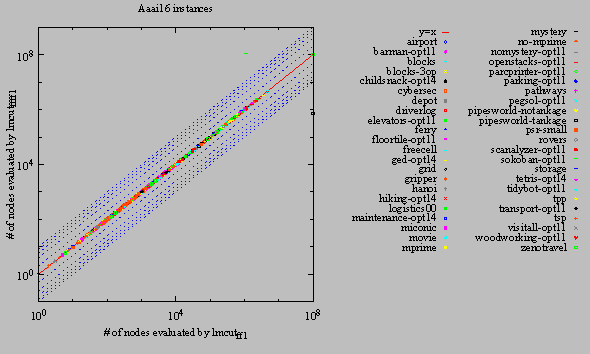
\includegraphics{tables/aaai16-evaluated-lmcut_ff-lmcut_ffff.pdf}
\linebreak
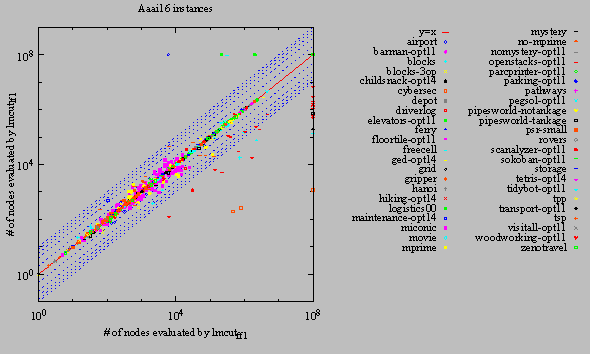
\includegraphics{tables/aaai16-evaluated-lmcut_ff-lmcut_lf.pdf}
\linebreak
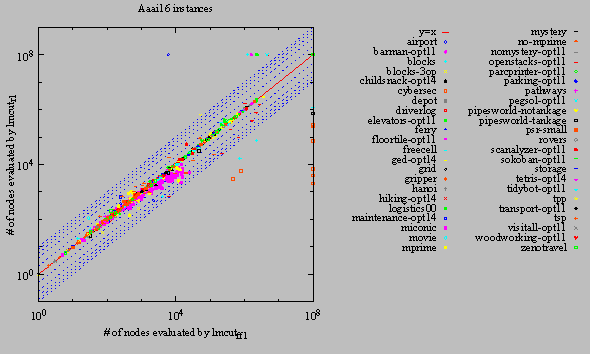
\includegraphics{tables/aaai16-evaluated-lmcut_ff-lmcut_r.pdf}
\linebreak
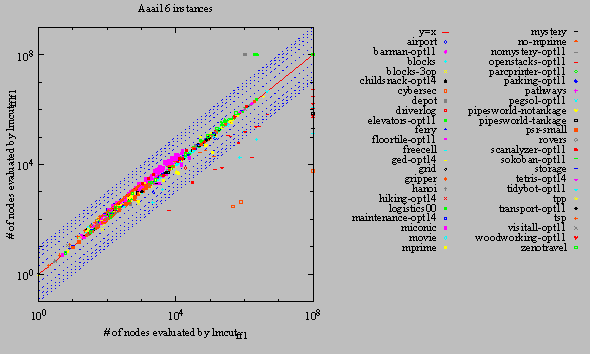
\includegraphics{tables/aaai16-evaluated-lmcut_ff-lmcut_fflf.pdf}
\linebreak
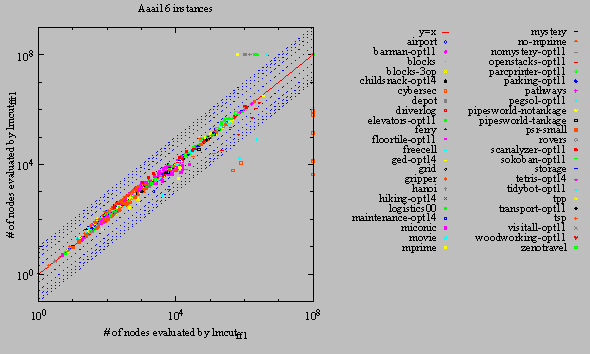
\includegraphics{tables/aaai16-evaluated-lmcut_ff-lmcut_ffr.pdf}
\linebreak
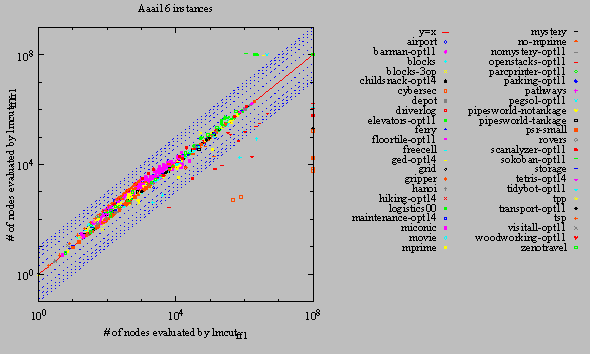
\includegraphics{tables/aaai16-evaluated-lmcut_ff-lmcut_fflfr.pdf}
\linebreak
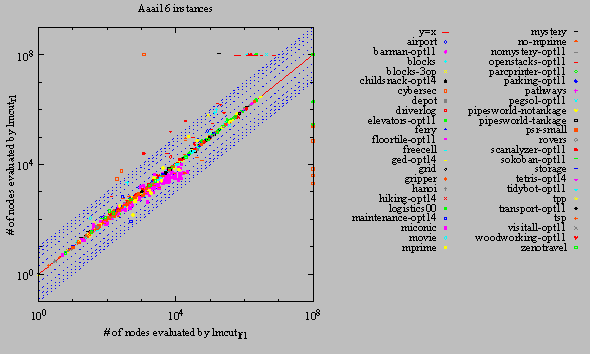
\includegraphics{tables/aaai16-evaluated-lmcut_lf-lmcut_r.pdf}
\linebreak
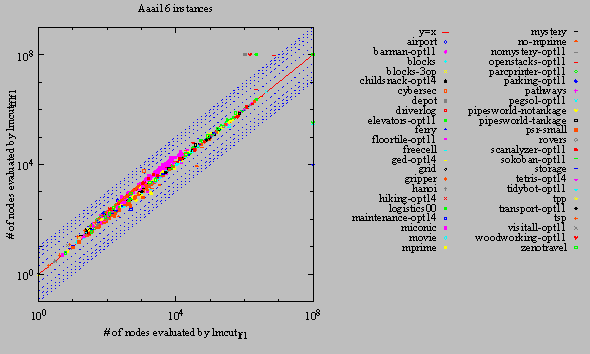
\includegraphics{tables/aaai16-evaluated-lmcut_lf-lmcut_fflf.pdf}
\linebreak
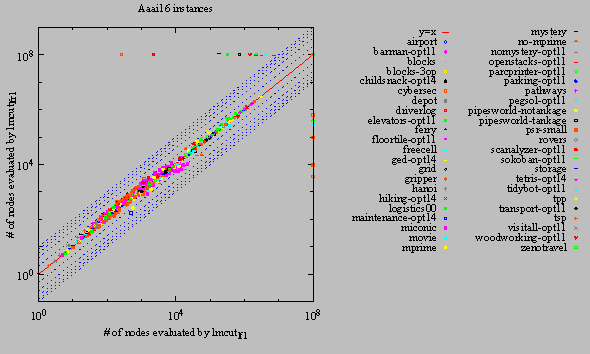
\includegraphics{tables/aaai16-evaluated-lmcut_lf-lmcut_lfr.pdf}
\linebreak
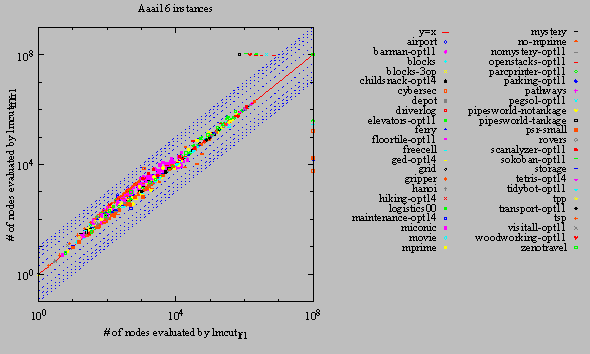
\includegraphics{tables/aaai16-evaluated-lmcut_lf-lmcut_fflfr.pdf}
\linebreak
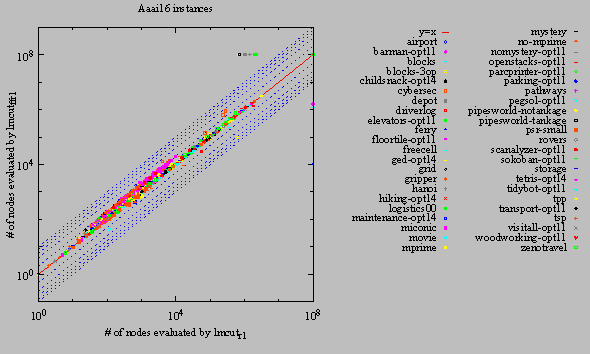
\includegraphics{tables/aaai16-evaluated-lmcut_r-lmcut_ffr.pdf}
\linebreak
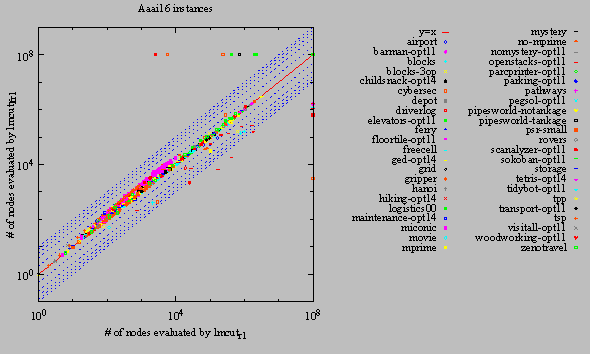
\includegraphics{tables/aaai16-evaluated-lmcut_r-lmcut_lfr.pdf}
\linebreak
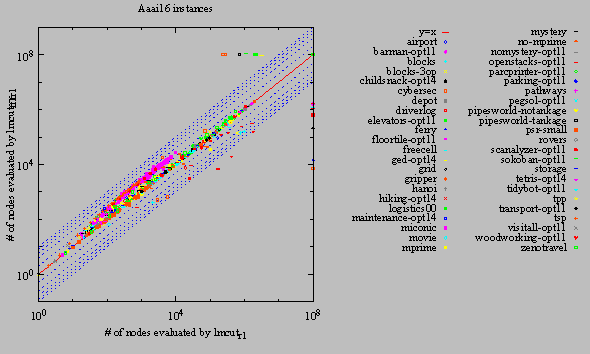
\includegraphics{tables/aaai16-evaluated-lmcut_r-lmcut_fflfr.pdf}
\linebreak

 \caption{Comparisons of \# of Evaluations between simple \lifo, \fifo,
 \ro second-level tiebreaking. Each line shows $\times 2,4,6\ldots$ boundary.}
 \label{f-h-eval}
\end{figure}

\refig{f-h-eval} gives us a more fine-grained analysis by comparing the
number of node evaluation (computations of \lmcut) on
different tiebreakings. We confirm that the difference between several
tiebreakings are sometime larger than $\times 10$.

In \reftbl{f-h-coverage}, we also added $[f,\fifo]$, $[f,\lifo]$ and
$[f,\ro]$ which does not use $h$-based first-level tiebreaking.
Interestingly, the coverage by LIFO-tiebreaking is almost comparable to
those with $h$-based tiebreaking, indicating that $h$-based tiebreaking
is not always necessary.  This is a surprising result considering
that almost all of the past literature assume the importance of the
$h$-based tiebreaking and modern forward search planners employ one.

Note that, although LIFO dominated the others, we consider this is just
by a coincidence due to our selection of problems, time limit and
domains. \emph{We are not trying to claim that any of LIFO or FIFO or
Random order dominates the other}. However, there are noticeable
performance difference caused by these different tiebreaking strategies.

\subsection{Size of the Plateau Matters}

We also observed that, such differences occur especially in the problems which
have the huge search plateau, i.e., the problems where the heuristic
function is not informative and the planner relies heavily on the
tiebreaking criteria.
% 
\refig{plateau} plots the size of the final search plateau with and
without $h$-based tiebreaking. In the first plot, $y$-axis shows the
number of nodes $f=f*, h=0$ and $x$-axis shows the total number of nodes
$f\leq f^*$.  In the second plot, $y$-axis shows the number of nodes
$f=f*$ (For $x$-axis, same as above.)  The size of the bucket does not
change between $[f,h,\fifo]$, $[f,h,\lifo]$ and $[f,h,\ro]$, or between
$[f,\fifo]$, $[f,\lifo]$ and $[f,\ro]$.

From this figure, in some domains, the planner cound spend most of the
runtime on searching through the final plateau in the worst case: The
goal node is evaluated in the very last iteration. It also means that
these domains have very large variance in the runtime caused by the
difference in second-level tiebreakings.  As expected, when the
$h$-based tiebreaking is disabled, much larger effort could be spent on
the final plateau.

\begin{figure}[htb]
 \centering \relsize{-3}
 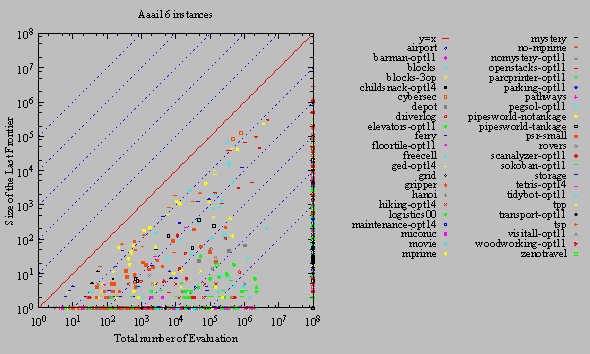
\includegraphics{tables/aaai16-front-vs-evaluated.pdf}
\linebreak
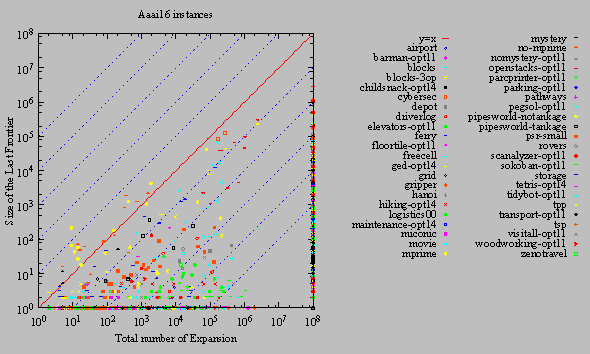
\includegraphics{tables/aaai16-front-vs-expanded.pdf}
\linebreak

 \caption{Comparison of the size of the search plateau compared to the
 total evaluation below $f\leq f^*$. Data were obtained by the result of standard FIFO
 tiebreaking on the standard benchmark instances. Both axes are
 logarithmic. Dotted lines represent $\times 10^n$ boundaries.
 Openstacks clearly has the large plateaus.}  \label{plateau}
\end{figure}

[Size of plateau on zerocost]

\subsection{Evaluating Depth-based Tiebreaking}

Next, we evaluated the 3 depth-based tiebreaking methods combined with 3
bucket implementations, resulting in 9 configurations.

Note that, the node evaluation order of $[\cdot,\fd,\fifo]$ and $[\cdot,\ld,\lifo]$
are exactly the same as those without the second-level
depth-based tiebreaking, i.e.\ $[\cdot,\fifo]$ and $[\cdot,\lifo]$.
Yet these results are useful in assessing the extra cost of managing the
depth-based buckets.

\refig{depth} shows various experiments on benchmark domains and
zerocost domains. Regardless of the third-level tiebreaking, LastDepth
strategy tends to be dominant in most domains. However, RandomDepth and
FirstDepth still exhibits a significantly better performance in Cybersec
and Mistery-Feast, respectively, indicating there is no true dominance relationship.

This result explains why the simple $[f,h,\lifo]$ strategy has
become successful. The fact that the performance of $[f,h,\ld,\cdot]$
was consistently good regardless of the third-level tiebreaking means
that the performance of $[f,h,\lifo]$ was actually caused by its
inherent LastDepth search pattern, and not by the implementation of LIFO
by themselves.

Supporting the above claim that the key is LastDepth and not LIFO, the
overall dominant third-level tiebreaking (in terms of coverage) is FIFO
when the second-level tiebreaking is the same.  For example, when we fix
the second-level tiebreaking, the coverages are
$[f,h,X,\fifo]>[f,h,X,\ro]>[f,h,X,\lifo]$ when $X=\ld,\rd$.
% 
Note that FIFO is bad in terms of low-level memory access
pattern since the insertion and deletion happens in the opposite side of
the bucket. It suggests that FIFO ordering is an order of magnitude
important in many domains compared to the low-level performance.
% 
Still, there does exist several domains where FIFO is not dominating
the others.
For example, in Pipesworld-Pushend, the dominant third-level strategy is
RandomOrder, regardless of the second-level depth tiebreaking.
(3,3,3 in FirstDepth, 3,4,3 in RandomDepth, and 5,6,4 in LastDepth.)

% 
% However, interestingly, in RandomDepth second-level tiebreaking, the
% RandomOrder third-level tiebreaking is good in Airport-Fuel and
% Mprime-Succumb.

% Although above result suggests that the depth-based tiebreaking and
% third-level tiebreaking affects the performance,
One issue in the above analysis is that this difference might
be caused by the accidental bias in the action order in the
domain definitions.
To address this issue, we also tested the zerocost domains
in which we mechanically shuffled the action orderings in the
domain file. The results showed the same trends as in the original
zerocost domains. (Due to space constraint, we put this figure in the
supplementaly material.)

Another issue in this result is the lack of analysis on
abstraction-based heuristics. We also added the results in the figures
in the supplemental materials. Above trends are mostly consistent when
M\&S and blind heuristics are used, regardless of first-level
tiebreaking by $h$-value. However, we note that many instances quickly
exhausted the 2GB memory limit with those heuristics, and is less
informative compared to the result by LMcut.

\begin{figure}[htb]
 \centering
 \relsize{-3}
 \begin{tabular}{|c|c|c|c||c|c|c|c|c|c|c|c|c|}
\hline                                    
 Domain & \rotatebox[origin=l]{90}{${\mbox{lmcut}}_{\mbox{ff}}$}   & \rotatebox[origin=l]{90}{${\mbox{lmcut}}_{\mbox{r}}$}   & \rotatebox[origin=l]{90}{${\mbox{lmcut}}_{\mbox{lf}}$}   & \rotatebox[origin=l]{90}{${\mbox{lmcut}}_{\mbox{${\mbox{fd}}_{\mbox{fifo}}$}}$}   & \rotatebox[origin=l]{90}{${\mbox{lmcut}}_{\mbox{${\mbox{rd}}_{\mbox{fifo}}$}}$}   & \rotatebox[origin=l]{90}{${\mbox{lmcut}}_{\mbox{${\mbox{ld}}_{\mbox{fifo}}$}}$}   & \rotatebox[origin=l]{90}{${\mbox{lmcut}}_{\mbox{${\mbox{fd}}_{\mbox{random}}$}}$}   & \rotatebox[origin=l]{90}{${\mbox{lmcut}}_{\mbox{${\mbox{rd}}_{\mbox{random}}$}}$}   & \rotatebox[origin=l]{90}{${\mbox{lmcut}}_{\mbox{${\mbox{ld}}_{\mbox{random}}$}}$}   & \rotatebox[origin=l]{90}{${\mbox{lmcut}}_{\mbox{${\mbox{fd}}_{\mbox{lifo}}$}}$}   & \rotatebox[origin=l]{90}{${\mbox{lmcut}}_{\mbox{${\mbox{rd}}_{\mbox{lifo}}$}}$}   & \rotatebox[origin=l]{90}{${\mbox{lmcut}}_{\mbox{${\mbox{ld}}_{\mbox{lifo}}$}}$}    \\
\hline                                    
 sum(1104) &  560 &  556 &  565 &  558 &  \textbf{568} &  \textbf{568} &  556 &  565 &  565 &  558 &  567 &  565  \\
\hline                                    
 {\relsize{-1}airport(50)} &  \textbf{27} &  25 &  26 &  \textbf{27} &  \textbf{27} &  \textbf{27} &  25 &  25 &  25 &  26 &  26 &  26  \\
 {\relsize{-1}cybersec(19)} &  1 &  2 &  2 &  1 &  \textbf{3} &  \textbf{3} &  2 &  \textbf{3} &  \textbf{3} &  2 &  \textbf{3} &  2  \\
 {\relsize{-1}mystery(30)} &  \textbf{16} &  15 &  \textbf{16} &  15 &  \textbf{16} &  \textbf{16} &  15 &  15 &  15 &  \textbf{16} &  \textbf{16} &  15  \\
 {\relsize{-1}openstacks-opt11(20)} &  12 &  10 &  \textbf{18} &  12 &  \textbf{18} &  \textbf{18} &  10 &  \textbf{18} &  \textbf{18} &  11 &  \textbf{18} &  \textbf{18}  \\
 {\relsize{-1}storage(30)} &  \textbf{15} &  \textbf{15} &  14 &  \textbf{15} &  \textbf{15} &  \textbf{15} &  \textbf{15} &  \textbf{15} &  \textbf{15} &  14 &  \textbf{15} &  \textbf{15}  \\
 {\relsize{-1}zenotravel(20)} &  \textbf{11} &  \textbf{11} &  \textbf{11} &  10 &  \textbf{11} &  \textbf{11} &  \textbf{11} &  \textbf{11} &  \textbf{11} &  \textbf{11} &  \textbf{11} &  \textbf{11} \\
\hline
 sum(380) &  163 &  163 &  166 &  163 &  175 &  \textbf{177} &  158 &  172 &  173 &  164 &  167 &  165  \\
\hline                                    
 {\relsize{-1}airport-fuel(20)} &  \textbf{15} &  14 &  14 &  \textbf{15} &  14 &  14 &  14 &  13 &  13 &  14 &  \textbf{15} &  14  \\
 {\relsize{-1}driverlog-fuel(20)} &  \textbf{8} &  \textbf{8} &  \textbf{8} &  \textbf{8} &  \textbf{8} &  7 &  \textbf{8} &  \textbf{8} &  7 &  \textbf{8} &  \textbf{8} &  7  \\
 {\relsize{-1}logistics00-fuel(28)} &  \textbf{16} &  15 &  \textbf{16} &  \textbf{16} &  \textbf{16} &  \textbf{16} &  15 &  15 &  15 &  \textbf{16} &  \textbf{16} &  \textbf{16}  \\
 {\relsize{-1}miconic-up(30)} &  16 &  17 &  18 &  16 &  \textbf{20} &  \textbf{20} &  15 &  \textbf{20} &  \textbf{20} &  16 &  18 &  18  \\
 {\relsize{-1}mprime-succumb(35)} &  15 &  16 &  14 &  15 &  21 &  \textbf{25} &  15 &  21 &  23 &  17 &  15 &  14  \\
 {\relsize{-1}pathways-fuel(30)} &  \textbf{5} &  \textbf{5} &  \textbf{5} &  \textbf{5} &  \textbf{5} &  4 &  4 &  4 &  4 &  \textbf{5} &  \textbf{5} &  \textbf{5}  \\
 {\relsize{-1}tpp-fuel(30)} &  8 &  8 &  \textbf{11} &  8 &  \textbf{11} &  \textbf{11} &  7 &  \textbf{11} &  \textbf{11} &  8 &  10 &  \textbf{11} \\
\hline
 sum(260) &  109 &  111 &  131 &  109 &  129 &  135 &  103 &  127 &  \textbf{137} &  110 &  127 &  130  \\
\hline                                    
 {\relsize{-1}blocks-stack(20)} &  17 &  17 &  17 &  17 &  17 &  \textbf{18} &  17 &  17 &  \textbf{18} &  17 &  17 &  17  \\
 {\relsize{-1}elevators-up(20)} &  7 &  6 &  \textbf{13} &  7 &  9 &  11 &  5 &  10 &  11 &  7 &  11 &  \textbf{13}  \\
 {\relsize{-1}freecell-move(20)} &  4 &  5 &  19 &  4 &  16 &  \textbf{20} &  4 &  16 &  \textbf{20} &  4 &  18 &  19  \\
 {\relsize{-1}gripper-move(20)} &  \textbf{7} &  6 &  \textbf{7} &  \textbf{7} &  \textbf{7} &  \textbf{7} &  6 &  6 &  6 &  \textbf{7} &  \textbf{7} &  \textbf{7}  \\
 {\relsize{-1}mystery-feast(20)} &  \textbf{8} &  7 &  6 &  \textbf{8} &  7 &  6 &  7 &  7 &  6 &  \textbf{8} &  7 &  6  \\
 {\relsize{-1}pipesnt-pushstart(20)} &  8 &  9 &  8 &  8 &  \textbf{10} &  \textbf{10} &  8 &  \textbf{10} &  \textbf{10} &  8 &  8 &  8  \\
 {\relsize{-1}pipesworld-pushend(20)} &  3 &  4 &  4 &  3 &  3 &  5 &  3 &  4 &  \textbf{6} &  3 &  3 &  4  \\
 {\relsize{-1}psr-small-open(20)} &  \textbf{19} &  18 &  \textbf{19} &  \textbf{19} &  \textbf{19} &  \textbf{19} &  18 &  \textbf{19} &  \textbf{19} &  \textbf{19} &  \textbf{19} &  \textbf{19}  \\
 {\relsize{-1}scanalyzer-analyze(20)} &  9 &  9 &  9 &  9 &  \textbf{10} &  9 &  9 &  9 &  9 &  \textbf{10} &  9 &  9  \\
 {\relsize{-1}sokoban-pushgoal(20)} &  \textbf{18} &  \textbf{18} &  \textbf{18} &  \textbf{18} &  \textbf{18} &  17 &  \textbf{18} &  \textbf{18} &  17 &  \textbf{18} &  \textbf{18} &  17  \\
 {\relsize{-1}storage-lift(20)} &  4 &  5 &  4 &  4 &  5 &  \textbf{6} &  4 &  4 &  5 &  4 &  4 &  4  \\
 {\relsize{-1}woodworking-cut(20)} &  5 &  7 &  7 &  5 &  8 &  7 &  4 &  7 &  \textbf{10} &  5 &  6 &  7 \\
\hline
 total(1744) &  832 &  830 &  862 &  830 &  872 &  \textbf{880} &  817 &  864 &  875 &  832 &  861 &  860 \\
\hline
\end{tabular}

 \caption{Experiments
 comparing the coverages of 9 configurations (3 depth-based strategy
 $\times$ 3 queue implementions). For the space reason, we omitted those
 domains whose results are the same. (Full results are available in the
 supplemental material.) Each cell denotes the problem solved with 30
 min, 2GB setting. \textbf{Boldface} denotes the case where it achieved
 the best result among configurations. Zerocost domains are named
 according to [original]-[name of nonzero action].}
 \label{depth}
\end{figure}

\begin{figure}[htb]
 \centering
 \relsize{-3}
 \begin{tabular}{|c|c|c|c||c|c|c|c|c|c|c|c|c|}
\hline                                    
 Domain & \rotatebox[origin=l]{90}{${\mbox{lmcut}}_{\mbox{${\mbox{ff}}_{\mbox{noh}}$}}$}   & \rotatebox[origin=l]{90}{${\mbox{lmcut}}_{\mbox{${\mbox{r}}_{\mbox{noh}}$}}$}   & \rotatebox[origin=l]{90}{${\mbox{lmcut}}_{\mbox{${\mbox{lf}}_{\mbox{noh}}$}}$}   & \rotatebox[origin=l]{90}{${\mbox{lmcut}}_{\mbox{${\mbox{fd}}_{\mbox{${\mbox{fifo}}_{\mbox{noh}}$}}$}}$}   & \rotatebox[origin=l]{90}{${\mbox{lmcut}}_{\mbox{${\mbox{rd}}_{\mbox{${\mbox{fifo}}_{\mbox{noh}}$}}$}}$}   & \rotatebox[origin=l]{90}{${\mbox{lmcut}}_{\mbox{${\mbox{ld}}_{\mbox{${\mbox{fifo}}_{\mbox{noh}}$}}$}}$}   & \rotatebox[origin=l]{90}{${\mbox{lmcut}}_{\mbox{${\mbox{fd}}_{\mbox{${\mbox{random}}_{\mbox{noh}}$}}$}}$}   & \rotatebox[origin=l]{90}{${\mbox{lmcut}}_{\mbox{${\mbox{rd}}_{\mbox{${\mbox{random}}_{\mbox{noh}}$}}$}}$}   & \rotatebox[origin=l]{90}{${\mbox{lmcut}}_{\mbox{${\mbox{ld}}_{\mbox{${\mbox{random}}_{\mbox{noh}}$}}$}}$}   & \rotatebox[origin=l]{90}{${\mbox{lmcut}}_{\mbox{${\mbox{fd}}_{\mbox{${\mbox{lifo}}_{\mbox{noh}}$}}$}}$}   & \rotatebox[origin=l]{90}{${\mbox{lmcut}}_{\mbox{${\mbox{rd}}_{\mbox{${\mbox{lifo}}_{\mbox{noh}}$}}$}}$}   & \rotatebox[origin=l]{90}{${\mbox{lmcut}}_{\mbox{${\mbox{ld}}_{\mbox{${\mbox{lifo}}_{\mbox{noh}}$}}$}}$}    \\
\hline                                    
 sum(1104) &  445 &  445 &  559 &  446 &  538 &  559 &  441 &  \textbf{564} &  \textbf{564} &  445 &  545 &  560  \\
\hline                                    
 {\relsize{-1}airport(50)} &  18 &  18 &  \textbf{26} &  18 &  21 &  25 &  18 &  21 &  \textbf{26} &  18 &  22 &  25  \\
 {\relsize{-1}blocks(35)} &  26 &  26 &  27 &  26 &  \textbf{28} &  \textbf{28} &  26 &  \textbf{28} &  26 &  26 &  27 &  27  \\
 {\relsize{-1}cybersec(19)} &  0 &  0 &  1 &  0 &  2 &  3 &  0 &  \textbf{4} &  \textbf{4} &  0 &  \textbf{4} &  2  \\
 {\relsize{-1}depot(22)} &  5 &  5 &  \textbf{6} &  5 &  \textbf{6} &  \textbf{6} &  5 &  \textbf{6} &  \textbf{6} &  5 &  \textbf{6} &  \textbf{6}  \\
 {\relsize{-1}driverlog(20)} &  12 &  12 &  \textbf{13} &  12 &  12 &  12 &  12 &  \textbf{13} &  \textbf{13} &  12 &  \textbf{13} &  \textbf{13}  \\
 {\relsize{-1}elevators-opt11(20)} &  14 &  14 &  \textbf{15} &  14 &  14 &  14 &  14 &  \textbf{15} &  \textbf{15} &  14 &  \textbf{15} &  \textbf{15}  \\
 {\relsize{-1}freecell(80)} &  8 &  \textbf{9} &  \textbf{9} &  \textbf{9} &  \textbf{9} &  \textbf{9} &  8 &  \textbf{9} &  \textbf{9} &  8 &  \textbf{9} &  \textbf{9}  \\
 {\relsize{-1}logistics00(28)} &  16 &  16 &  19 &  16 &  \textbf{20} &  \textbf{20} &  16 &  \textbf{20} &  \textbf{20} &  16 &  19 &  19  \\
 {\relsize{-1}miconic(150)} &  68 &  68 &  \textbf{140} &  68 &  126 &  \textbf{140} &  68 &  \textbf{140} &  \textbf{140} &  68 &  125 &  \textbf{140}  \\
 {\relsize{-1}mprime(35)} &  20 &  19 &  \textbf{22} &  20 &  \textbf{22} &  \textbf{22} &  20 &  21 &  21 &  20 &  \textbf{22} &  \textbf{22}  \\
 {\relsize{-1}mystery(30)} &  15 &  15 &  \textbf{16} &  15 &  \textbf{16} &  \textbf{16} &  15 &  \textbf{16} &  \textbf{16} &  15 &  \textbf{16} &  \textbf{16}  \\
 {\relsize{-1}nomystery-opt11(20)} &  12 &  12 &  13 &  12 &  12 &  12 &  12 &  \textbf{14} &  \textbf{14} &  12 &  13 &  \textbf{14}  \\
 {\relsize{-1}openstacks-opt11(20)} &  12 &  10 &  \textbf{18} &  12 &  \textbf{18} &  \textbf{18} &  10 &  \textbf{18} &  \textbf{18} &  12 &  \textbf{18} &  \textbf{18}  \\
 {\relsize{-1}parcprinter-opt11(20)} &  12 &  12 &  \textbf{13} &  12 &  \textbf{13} &  \textbf{13} &  12 &  \textbf{13} &  \textbf{13} &  12 &  \textbf{13} &  \textbf{13}  \\
 {\relsize{-1}pathways(30)} &  4 &  4 &  \textbf{5} &  4 &  \textbf{5} &  \textbf{5} &  4 &  \textbf{5} &  \textbf{5} &  4 &  \textbf{5} &  \textbf{5}  \\
 {\relsize{-1}pegsol-opt11(20)} &  \textbf{17} &  16 &  \textbf{17} &  \textbf{17} &  \textbf{17} &  \textbf{17} &  16 &  \textbf{17} &  \textbf{17} &  \textbf{17} &  \textbf{17} &  \textbf{17}  \\
 {\relsize{-1}pipesworld-notankage(50)} &  13 &  13 &  13 &  13 &  13 &  13 &  13 &  \textbf{15} &  \textbf{15} &  13 &  13 &  13  \\
 {\relsize{-1}pipesworld-tankage(50)} &  7 &  \textbf{8} &  \textbf{8} &  7 &  \textbf{8} &  \textbf{8} &  7 &  \textbf{8} &  \textbf{8} &  7 &  \textbf{8} &  \textbf{8}  \\
 {\relsize{-1}scanalyzer-opt11(20)} &  4 &  4 &  \textbf{10} &  4 &  9 &  \textbf{10} &  4 &  9 &  \textbf{10} &  4 &  9 &  \textbf{10}  \\
 {\relsize{-1}storage(30)} &  14 &  14 &  14 &  14 &  14 &  14 &  14 &  \textbf{15} &  \textbf{15} &  14 &  14 &  14  \\
 {\relsize{-1}tidybot-opt11(20)} &  11 &  11 &  \textbf{12} &  11 &  11 &  11 &  11 &  \textbf{12} &  \textbf{12} &  11 &  \textbf{12} &  \textbf{12}  \\
 {\relsize{-1}visitall-opt11(20)} &  \textbf{10} &  \textbf{10} &  \textbf{10} &  \textbf{10} &  \textbf{10} &  \textbf{10} &  9 &  \textbf{10} &  \textbf{10} &  \textbf{10} &  \textbf{10} &  \textbf{10}  \\
 {\relsize{-1}woodworking-opt11(20)} &  6 &  8 &  9 &  6 &  9 &  10 &  6 &  \textbf{12} &  8 &  6 &  \textbf{12} &  9  \\
 {\relsize{-1}zenotravel(20)} &  9 &  9 &  \textbf{11} &  9 &  \textbf{11} &  \textbf{11} &  9 &  \textbf{11} &  \textbf{11} &  9 &  \textbf{11} &  \textbf{11} \\
\hline
 sum(380) &  137 &  130 &  167 &  137 &  165 &  \textbf{172} &  133 &  169 &  170 &  139 &  164 &  166  \\
\hline                                    
 {\relsize{-1}airport-fuel(20)} &  7 &  7 &  \textbf{15} &  7 &  10 &  14 &  8 &  10 &  14 &  8 &  12 &  \textbf{15}  \\
 {\relsize{-1}depot-fuel(22)} &  5 &  5 &  \textbf{6} &  5 &  \textbf{6} &  \textbf{6} &  5 &  \textbf{6} &  \textbf{6} &  5 &  \textbf{6} &  \textbf{6}  \\
 {\relsize{-1}driverlog-fuel(20)} &  7 &  5 &  \textbf{8} &  7 &  \textbf{8} &  6 &  6 &  \textbf{8} &  5 &  7 &  7 &  7  \\
 {\relsize{-1}ged-opt14(20)} &  \textbf{15} &  14 &  \textbf{15} &  \textbf{15} &  13 &  13 &  13 &  \textbf{15} &  14 &  \textbf{15} &  \textbf{15} &  \textbf{15}  \\
 {\relsize{-1}hiking-fuel(20)} &  8 &  8 &  \textbf{9} &  8 &  \textbf{9} &  \textbf{9} &  8 &  \textbf{9} &  \textbf{9} &  8 &  \textbf{9} &  \textbf{9}  \\
 {\relsize{-1}logistics00-fuel(28)} &  15 &  15 &  \textbf{16} &  15 &  \textbf{16} &  15 &  15 &  15 &  15 &  15 &  \textbf{16} &  \textbf{16}  \\
 {\relsize{-1}miconic-up(30)} &  10 &  10 &  18 &  10 &  \textbf{20} &  \textbf{20} &  10 &  19 &  18 &  10 &  19 &  18  \\
 {\relsize{-1}mprime-succumb(35)} &  12 &  9 &  14 &  12 &  21 &  \textbf{25} &  11 &  20 &  23 &  13 &  14 &  14  \\
 {\relsize{-1}nomystery-fuel(20)} &  9 &  9 &  \textbf{10} &  9 &  9 &  9 &  9 &  \textbf{10} &  \textbf{10} &  9 &  \textbf{10} &  \textbf{10}  \\
 {\relsize{-1}pathways-fuel(30)} &  4 &  4 &  \textbf{5} &  4 &  4 &  4 &  4 &  \textbf{5} &  4 &  4 &  \textbf{5} &  \textbf{5}  \\
 {\relsize{-1}rovers-fuel(40)} &  7 &  7 &  \textbf{9} &  7 &  8 &  \textbf{9} &  7 &  \textbf{9} &  \textbf{9} &  7 &  \textbf{9} &  \textbf{9}  \\
 {\relsize{-1}tidybot-motion(20)} &  14 &  14 &  15 &  14 &  15 &  15 &  14 &  \textbf{16} &  \textbf{16} &  14 &  \textbf{16} &  15  \\
 {\relsize{-1}tpp-fuel(30)} &  8 &  7 &  \textbf{11} &  8 &  10 &  \textbf{11} &  7 &  \textbf{11} &  \textbf{11} &  8 &  10 &  \textbf{11} \\
\hline
 sum(260) &  92 &  96 &  129 &  92 &  122 &  133 &  89 &  129 &  \textbf{139} &  92 &  121 &  128  \\
\hline                                    
 {\relsize{-1}blocks-stack(20)} &  15 &  15 &  17 &  15 &  17 &  \textbf{18} &  15 &  17 &  \textbf{18} &  15 &  17 &  17  \\
 {\relsize{-1}elevators-up(20)} &  7 &  6 &  \textbf{13} &  7 &  9 &  11 &  6 &  10 &  11 &  7 &  11 &  \textbf{13}  \\
 {\relsize{-1}freecell-move(20)} &  4 &  5 &  19 &  4 &  16 &  \textbf{20} &  4 &  16 &  \textbf{20} &  4 &  18 &  19  \\
 {\relsize{-1}gripper-move(20)} &  \textbf{7} &  6 &  \textbf{7} &  \textbf{7} &  \textbf{7} &  \textbf{7} &  6 &  6 &  6 &  \textbf{7} &  \textbf{7} &  \textbf{7}  \\
 {\relsize{-1}mystery-feast(20)} &  5 &  6 &  5 &  5 &  6 &  5 &  5 &  6 &  6 &  5 &  \textbf{7} &  5  \\
 {\relsize{-1}pipesnt-pushstart(20)} &  6 &  8 &  7 &  6 &  9 &  9 &  6 &  \textbf{10} &  \textbf{10} &  6 &  6 &  7  \\
 {\relsize{-1}pipesworld-pushend(20)} &  2 &  3 &  4 &  2 &  2 &  4 &  2 &  5 &  \textbf{7} &  2 &  4 &  3  \\
 {\relsize{-1}psr-small-open(20)} &  \textbf{19} &  18 &  \textbf{19} &  \textbf{19} &  \textbf{19} &  \textbf{19} &  18 &  \textbf{19} &  \textbf{19} &  \textbf{19} &  \textbf{19} &  \textbf{19}  \\
 {\relsize{-1}scanalyzer-analyze(20)} &  3 &  3 &  9 &  3 &  7 &  9 &  3 &  8 &  \textbf{10} &  3 &  3 &  9  \\
 {\relsize{-1}sokoban-pushgoal(20)} &  \textbf{18} &  \textbf{18} &  \textbf{18} &  \textbf{18} &  \textbf{18} &  17 &  \textbf{18} &  \textbf{18} &  17 &  \textbf{18} &  \textbf{18} &  17  \\
 {\relsize{-1}storage-lift(20)} &  4 &  4 &  4 &  4 &  5 &  \textbf{7} &  4 &  5 &  5 &  4 &  5 &  5  \\
 {\relsize{-1}woodworking-cut(20)} &  2 &  4 &  7 &  2 &  7 &  7 &  2 &  9 &  \textbf{10} &  2 &  6 &  7 \\
\hline
 total(1744) &  674 &  671 &  855 &  675 &  825 &  864 &  663 &  862 &  \textbf{873} &  676 &  830 &  854 \\
\hline
\end{tabular}

 \caption{Same experiments without first-level tiebreaking by $h$-value.}
 \label{depth-noh}
\end{figure}


\subsection{Evaluating MultiSearch Strategy}

As we see in the previous section, the planner performance is greatly
affected by the tiebreaking criteria, especially when the search plateau
is huge. Therefore, the multisearch strategy should avoid the
worst-case scenario caused by bad tiebreaking, and quickly find the solution.

First, we show that the doubled cost of insertion and deletion by
MultiSearch is negligeble.  
We verified this by running a MultiSearch search engine with two same search engines, each using \lmcut and FIFO queue, and compared its runtime agains the single engine using \lmcut and FIFO. The result in \refig{ffff} shows that the extra cost of duplicated effort is negligeble.

\begin{figure}[htbp]
 \centering
 \relsize{-2}
 % 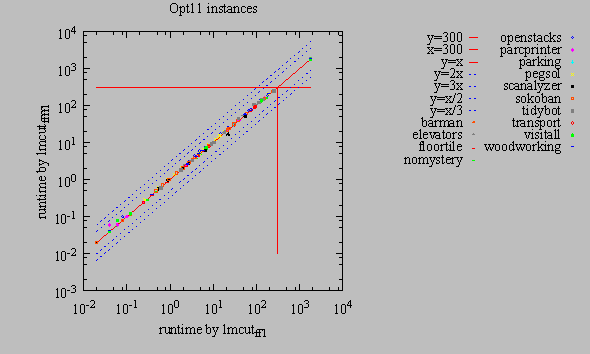
\includegraphics{tables/opt11-time-lmcut_ff-lmcut_ffff.pdf}
 \caption{Comparison of runtime on problems solved by both single FIFO search engine (ff) and a MultiSearch engine with 2 different instances of the same FIFO engine (ffff). The runtime difference was on average below a factor of x1.1, if we ignore the subsecond differences.}
 \label{ffff}
\end{figure}

Next, we conducted experiments for evaluating our MultiSearch
strategy in order to show that it acutally follows the expected search
behavior and the theoretical bounds.
% , and also to show that it performs
% significantly better than its worst case $n \times \min$ performance.
\refig{portfolio} shows the runtime between
different combinations of 2 or 3 tiebreaking strategies (FIFO+LIFO,
FIFO+Random, LIFO+Random, FIFO+LIFO+Random) and the single tiebreaking
strategies. The results support our claim that the evaluation never
exceeds twice/thirds of the single search engine and, in practice, the
evaluations are mostly the same with the single search engine, and in
some domains with large plateaus, the search effort used by MultiSearch
is more than ten times less than by the worst single strategy.



\begin{figure}[htbp]
 \centering
 \relsize{-2}
 % 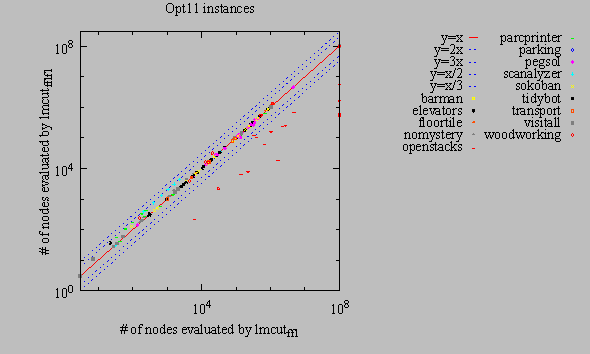
\includegraphics{tables/opt11-evaluated-lmcut_ff-lmcut_fflf.pdf}
 % 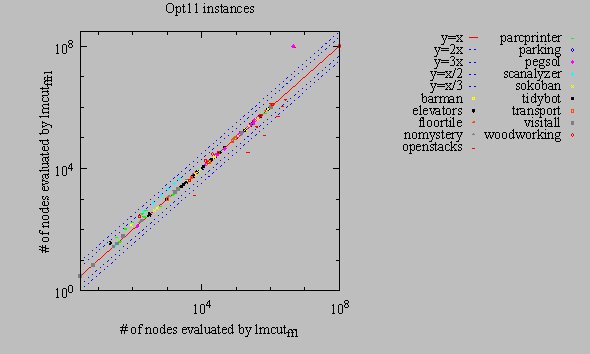
\includegraphics{tables/opt11-evaluated-lmcut_ff-lmcut_ffr.pdf}
 % 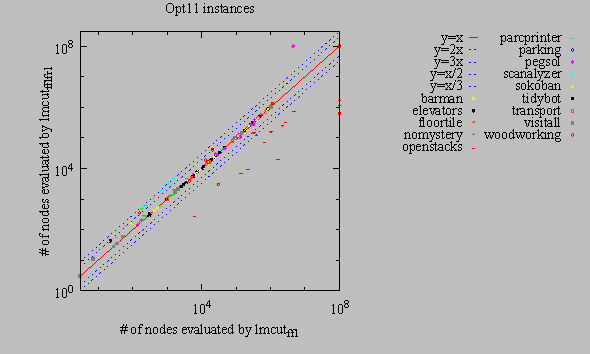
\includegraphics{tables/opt11-evaluated-lmcut_ff-lmcut_fflfr.pdf}
 \caption{}
 \label{portfolio}
\end{figure}


\section{Related Work}
\label{sec-4}

% Moved -- PLUSONE is for satisficing planning, and not directly related to tiebreaking
Another related techinques are found in the context of satisficing planning.
An inadmissible search technique in LAMA planner \cite{richter2010lama}
increases every action costs by 1, called \emph{PLUSONE} cost-type.
It is explicitly targeted at zero-cost actions observed in Openstacks,
and resulted in a significantly better performance in IPC-6.
In PLUSONE, three successive
applications of zero-cost operators result in cost 3, and two
applications result in a cost 2, and smaller cost is preferred, just as
\astar always expands the node with smaller $f$-value.
% Moved
The major difference of our depth-based tiebreaking from PLUSONE
strategy in LAMA is twofold.  First, the depth used for tiebreaking does
not affect the cost, thus our algorithm does not lose the
admissibility. Next, \emph{we do not always favor smaller depth over
larger depth}. LAMA's PLUSONE treats the increased cost as the part of
sorting criteria. It happens only in FirstDepth configuration.

The major difference of our depth-based tiebreaking from PLUSONE
strategy in LAMA is twofold.  First, the depth used for tiebreaking does
not affect the cost, thus does not lose the admissibility. Next, we
\emph{do not favor smaller depth over higher depth}. LAMA's PLUSONE
treats the increased cost as the part of sorting criteria. 

Another technique in LAMA is \emph{preferred operator queue},
which is a technique that favors those actions which decreased the
smallest $h$ value during the search.


\emph{Symmetry Breaking}
\cite{Fox1998,pochter2011exploiting,domshlak2013symmetry} is the search
technique that tries to prune the states with symmetric
paths. \emph{Partial Order Reduction}, \emph{Strong Stubbern Sets} and
\emph{Expansion Core} are also the techniques which prune the
intermediate states that reach to the same goal using the different
orders of same actions. \emph{Dominance Pruning} \cite{hall2013faster} is a
technique which prunes a state if it can be proven to be worse than the other nodes.
% 
\emph{Path-dependent globally admissible
heurisitics} \cite{karpas2012optimal} is a class of heuristics which is
admissible only on a particular optimal path, and generalizes the above
techniques because pruning a node is equivalent to assigining an
infinite cost to some nodes on the other optimal paths (thus, not
per-state admissible).
From a slightly different category, Pathmax \cite{mero1984heuristic} and
Bidirectional Pathmax \cite{felner2011inconsistent} are the techniques
which converts an inconsistent heuristics into non-decreasing,
consistent heuristics.
All of these methods are the
attempt to improve the heuristic estimates. Although in some particular
case they may be able to return a perfect heuristics, they are still not
always a perfect heuristics, implying that the plateau is unavoidable.
In contrast, our tiebreaking techniques aims specifically at the case
where the plateau is encountered and the planners are forced to run a
knowledge-free search.

$LA^*$ \cite{stern2010look} is an extension of \astar which employs a
\emph{lookahead} to each expansion of a node. Lookahead is a depth first
search from the frontier node limited to a particular depth $k$. When
$k=0$, called $LA^*_0$ in their paper, the greedy expansion reaches only within
the same $f$-value. It is the same as LastDepth strategy in our
case, but there is no mention comparing $LA^*_0$ to tiebreaking strategy.

In the realm of inadmissible search, the work on escaping the plateau is
abundant. DBFS \cite{imai2011novel} is a technique which stochastically
backtracks Greedy Best First Search to avoid being misdirected by the
heuristic function. Type based bucket \cite{xie14type} is an attempt to
classify the plateau of GBFS according to the $[g,h]$ pair.
Marvin \cite{Coles07} learns plateau-escaping macros from the Enhanced
Hill Climbing phase of the FF planner \cite{Hoffmann01} and later uses
these macros to escape the plateau.  However, to our knowledge, the
similar research on optimal planning was hardly located.

\section{Conclusion}

In this paper, we proposed two novel tie-braking methods for the admissible search using \astar. We empirically showed that they improve the performance on various domains, and they are heuristic-agnostic improvements. We showed that they have a significant impact on the final step of the search in large plateau.
 % when the distribution of optimal solutions is not uniform within the open list.
% We also showed that this nonuniform distribution still appears when we have almost-perfect % heuristics.

Our method differs from the pruning techniques because we actually
do not prune any states, nor from the other general improvements to the
heuristic accuracy because we just change the evaluation order within the
same $f$, yet it address the fundamental problems in the limitation of
heuristic forward search.  Future work includes a development of learning
technique for adaptively altering the search behavior in the plateau.



